% ED-11 -- The Rytova-Keldysh interaction is a positive Gaussian mixture
% Sources: TOP20.json pick 10; papers/ar_keldysh_tmd/{AUDIT.md,REVISION.md,publication_meta.json,main.tex,gen_numbers.tex}
% Figure: code/fig10.py -> figures/c10_keldysh.{pdf,png}
\chapter[Une force en tas de sable]{La force dans un semi-conducteur atomiquement mince, en tas de sable}
\reference{Préprint du 25 octobre 2026.\\ doi:10.5281/\\zenodo.23646107}

\section*{L'idée en une image}

\begin{analogie}
Prenez des tas de sable en forme de cloche, tous centrés au même endroit, certains étroits et hauts, d'autres larges
et plats. En les empilant, vous obtenez un profil compliqué. Un résultat déjà établi dit que \emph{chaque} cloche
obéit à une règle, et que toute pile obtenue en \emph{ajoutant} des cloches y obéit aussi. Le travail consiste à
montrer que la force étudiée est une telle pile, avec des quantités de sable toutes positives~: on n'a jamais le
droit d'\og enlever\fg{} du sable.

\emph{Où l'image cesse d'être juste~:} il faut ici une infinité continue de cloches, et l'égalité \og la force
physique est cette pile\fg{} n'a été démontrée qu'à la main~; le logiciel n'a vérifié que la pile elle-même.
\end{analogie}

\section*{Ce qui a été fait}

Dans un semi-conducteur atomiquement mince, une monocouche comme le disulfure de molybdène, deux charges ne
s'attirent ou ne se repoussent pas selon la loi de Coulomb habituelle. La couche, très polarisable, écrante la force
à courte distance~; de loin, on retrouve la loi en $1/r$. Cette loi modifiée, dite de Rytova--Keldysh, s'écrit avec
des fonctions spéciales et dépend d'une longueur $r_0$, propre au matériau.

L'article donne une preuve humaine, pas à pas, que cette force est un empilement positif de cloches (des
gaussiennes) de toutes les largeurs, avec un poids explicite. Dans Lean, il démontre trois choses~: tout empilement
positif de ce genre (avec des moyennes finies) a la propriété exigée par le théorème amont~; le potentiel
\emph{défini} par l'empilement l'a donc, ainsi qu'une version légèrement adoucie à grande distance~; et le réseau
triangulaire en découle comme arrangement d'énergie minimale, sous réserve du théorème amont.

\begin{encadre}
\textbf{À faire avec un crayon.} Pourquoi exiger des poids positifs~? Prenez deux cloches, écrites en
fonction de $t=r^2$, $e^{-t}$ et $e^{-2t}$.
\begin{itemize}
\item Avec des poids positifs, $e^{-t}+2e^{-2t}$ est toujours positif, et sa pente $-e^{-t}-4e^{-2t}$ toujours
  négative~: la répulsion décroît bien.
\item Avec un poids négatif, $e^{-t}-2e^{-2t}$~: en $t=\ln\frac32$, on a $e^{-t}=\frac23$ et $e^{-2t}=\frac49$, donc
  $\frac23-\frac89=-\frac29<0$. Une \og répulsion\fg{} qui devient négative~: la règle tombe. C'est exactement la
  contre-épreuve que Lean démontre dans l'article.
\end{itemize}
La figure~\ref{fig:c10} montre, à gauche, que l'écriture classique et l'empilement donnent la même courbe, et, à
droite, que tous les poids sont positifs.
\end{encadre}

Côté calcul (\niveau{X}), un module Rust du solveur rusty-SUNDIALS calcule l'énergie d'électrons rangés en réseau
avec cette force. Le réseau carré reste au-dessus du triangulaire aux 51 points essayés. Pour le disulfure de
molybdène dans le vide, à $10^{11}$ électrons par cm$^2$, l'écart vaut $0{,}431$~meV par électron.

\begin{figure}[htbp]
\centering
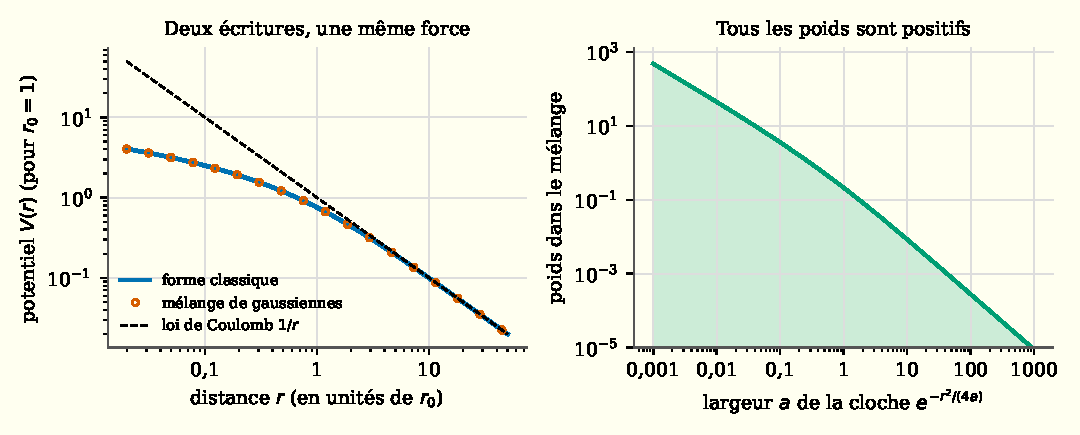
\includegraphics[width=\linewidth]{figures/c10_keldysh}
\caption{Formule classique et empilement de gaussiennes coïncident (gauche)~; les poids sont tous positifs (droite).}
\label{fig:c10}
\end{figure}

\section*{Comment on s'est assuré que ce n'est pas faux}

En résumé~: \niveau{C} pour l'identité \og c'est un mélange positif de gaussiennes\fg{} (preuve humaine),
\niveau{A} pour l'admissibilité du potentiel défini par ce mélange et pour les corollaires (conditionnels au
théorème amont), \niveau{X} pour les énergies calculées.

Pour les énoncés Lean, \og le juge a regardé\fg~: le noyau de Lean, le petit programme qui contrôle chaque pas logique,
les a acceptés avec seulement trois axiomes standard, et le rejeu du 26 octobre 2026 les a repassés sans erreur. Au
stade de l'article, producteur et vérificateur n'étaient pas séparés~; un auditeur distinct, un agent d'IA, a ensuite tout recompilé dans son propre répertoire et planté deux fausses preuves (un trou, un axiome
inventé), toutes deux dénoncées. Il a relancé le calcul Rust~: résultat identique au bit près.

Deux épisodes de cet audit valent d'être racontés. D'abord, une phrase de l'article, par une coquille de mise en
page, se lisait \og l'étape~7 n'est pas de niveau~C\fg, ce qui inversait son propre classement~; elle a été corrigée.
Ensuite, l'auditeur a proposé une preuve humaine plus simple, où n'interviennent que des quantités positives~;
elle est devenue la preuve principale, et reste au niveau \og un humain a raisonné\fg, faute d'outils dans la bibliothèque Lean pour
ces fonctions spéciales. Le registre reste marqué \og non audité\fg~: aucun humain n'a relu les énoncés.

\section*{Ce que ça ne dit pas}

\begin{limite}
\begin{itemize}
\item L'identité avec la formule physique est une preuve à la main (\niveau{C}), non vérifiée par la machine.
\item Comme la force décroît en $1/r$, la somme sur un réseau infini diverge~: l'inégalité brute doit se lire
  \og infini $\leq$ infini\fg{} et ne dit rien d'utile. Pour la version adoucie, la finitude de l'énergie n'est
  pas démontrée.
\item Tout est conditionnel au théorème amont, généré par une IA et non relu par des pairs.
\item Les énergies calculées sont statiques et classiques, et ne comparent que deux réseaux. La longueur $r_0$ de
  chaque matériau vient de la littérature (\niveau{L}).
\item La nouveauté est modeste~: la complète monotonie découle vite d'intégrales de manuel.
\end{itemize}
\end{limite}

\section*{Pour aller plus loin}

L'article, son registre et l'audit sont déposés sous doi:10.5281/\allowbreak zenodo.23646107. C'est l'exemple le plus net, dans
ce livre, de deux niveaux de confiance tenus séparés à l'intérieur d'un même résultat.
